

\documentclass[a4paper]{article}

\usepackage{color}
\usepackage{url}
\usepackage[T2A]{fontenc} 
\usepackage[utf8]{inputenc} 
\usepackage{graphicx}


\usepackage[english,serbian]{babel}


\usepackage[unicode]{hyperref}
\hypersetup{colorlinks,citecolor=green,filecolor=green,linkcolor=blue,urlcolor=blue}


\newtheorem{primer}{Primer}[section]

\begin{document}

\begin{titlepage}

\newcommand{\HRule}{\rule{\linewidth}{0.4mm}}

\center 
	
\textsc{\LARGE Matematički fakultet}\\[3cm] 
	
\textsc{\Large Seminarski rad}\\[0.1cm]
	
\textsc{\large iz uvoda u informatiku}\\[0.5cm] 
	
\HRule\\[0.4cm]
	
{\LARGE\bfseries "ILOVEYOU" malver}\\[0.2cm] 
	
\HRule\\[2cm]

\vspace{17\baselineskip}
		

	
	\begin{minipage}{0.4\textwidth}
		\begin{flushleft}
			\large
			\textit{Student}\\
			Ognjen Stefanović 66/2024
		\end{flushleft}
	\end{minipage}
\hspace*{1cm}
	\begin{minipage}{0.4\textwidth}
		\begin{flushright}
			\large
			\textit{Profesor}\\
			Danijela Simić
		\end{flushright}
	\end{minipage}
	
	
\vfill\vfill\vfill\vfill 
	
{\large Beograd, \today} 
	
\vfill 
	
\end{titlepage}

\tableofcontents

\newpage

\abstract{
Četvrtog maja 2000. godine je krenula pandemija "ljubavnog pisma", koji je za nedelju dana zarazio čak 45 miliona računara u 20 država i izazvao štetu između 7 i 10 milijarde dolara\cite{sprinkel2001global}. Za svu tu štetu je zaslužan mladić sa Filipina koji je poslao datoteku u Aziji, koja se brzo proširila u Evropi kasnije i u Americi. Ovaj malver je sposoban obriše bitne datoteke, da otvori veb pretraživač i instalira program koji sve šifre sa uređaja objavljuje na anoniman sajt, i za kraj prosledi svima iz imenika imejla originalan mejl. U ovom radu je opisano kako "bezopasno" pismo inficiralo organizacije od majkrosofta sve do pentagona.}


\section{Uvod}
\label{sec:uvod}
Sve je krenulo kada student računarskog fakulteta na Filipinima, Onel de Guzman, nije imao novca i mučio se sa plaćanjem računa za internet. U vreme dial-up interneta, korisnik je morao imati šifru da bi imao internet konekciju. Došao je na ideju da napravi virus koji će ukrasti šifre se uređaja žrtve i poslati njemu. Tada na Filipinima nije postojao zakon protiv sajber kriminala. Virus je poslat samo Filipincima sa kojima je razgovarao na internetu u čet-rumovijma (chat rooms) da bi im ukrao šifru za interenet. 
Ali četvrtog maja 2000. godine je uveo izmenu u kodu ,koristeći grešku u operativnom sistemu "Windows 95", da se imejl pošalje svim kontaktima žrtve. Dao je naziv datoteci "ILOVEYOU" jer je pretpostavio da svako hoće ljubav. Nakon poslatog imejla nekome u Singapuru otišao je na piće sa prijateljima. Saznao je da je nastala pandemija kada ga je majka pozvala da traže hakera u Manili\cite{bbc}. 

Korisnici su dobijali sledeći imejl:
\begin{figure}[h!]
\begin{center}
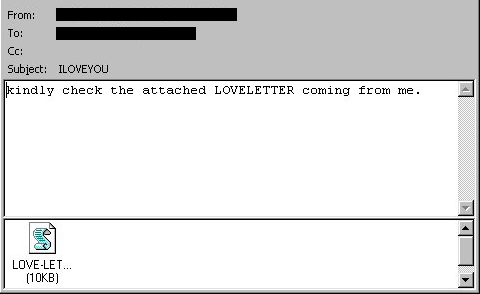
\includegraphics[scale=0.63]{slike/Primer_pisma.png}
\end{center}
\caption{Imejl sa inficiranom datotekom}
\end{figure}


\section{Struktura virusa}
Virus je napisan na Visual Basic programskom jeziku. Program se sastoji iz četiri glavne rutine, i prve koja ih poziva.\cite{bishop2000analysis} Rutine su:
\begin{itemize}
\item MAIN
\item REGRUNS
\item HTML
\item SPREADTOEMAIL
\item LISTADRIV
\end{itemize} 


\subsection{MAIN}
Main rutina kopira kod pisma na 3 mesta:
\begin{itemize}
\item \verb|root_folder\MSKernel32.vbs|
\item \verb|root_folder\LOVE-LETTER-FOR-YOU.TXT.vbs|
\item \verb|system_folder\Win32DLL.vbs|
\end{itemize}
Nakon toga, rutina main poziva regruns, html, spreadtoemail, listadriv.

\subsection{REGRUNS}

Regruns postavlja sledeće ključeva registra:
\begin{itemize}
\item \verb|HKEY_LOCAL_MACHINE\Software\Microsoft\Windows\|
\\ \verb|CurrentVersion\Run\MSKernel32| u \verb|system_folder\MSKernel32.vbs|
\item \verb|HKEY_LOCAL_MACHINE\Software\Microsoft\Windows\CurrentVersion\|
\\ \verb|RunServices\Win32DLL| u \verb|system_folder\Win32DLL.vbs|
\end{itemize}

Ako postoji datoteka \verb|temp_folder\WIN-BUGSFIX.exe|, postavlja ključ registra \verb|HKEY_LOCAL_MACHINE\Software\Microsoft\Windows\CurrentVersion\|
\\ \verb|Run\WIN-BUGSFIX | u tu datoteku i postavlja početnu stranu "Internet Explorer"-a na praznu stranu. 

Ova rutina ubacuje trojanske konje u sistem. Prvi trojanski konj je samo pismo koje se pokrece kada se pokrene računar. Drugi će biti učitan u sistem kada "Internet Explorer" učita svoju stranicu sa svetske mreže. Ako je već učitan, treći trojanski konj se takođe pokreće na pokretanju računara, i sada je početna strana veb pregledača prazna.


\subsection{HTML}

Rutina html kreira veb stranicu pod nazivom \\ \verb|system_folder\LOVE-LETTER-FORYOU.HTM|.
Ova stranica sadrži Java program koji kreira prozor i Visual Basic program koji rekreira pismo i pokreće ga. Ova stranica se koristi u rutini \verb|spreadtoemail|.

\subsection{SPREADTOEMAIL}
Ova rutina salje pismo svim korisnicima u imeniku žrtve. Za svaku adresu kreira kreira ključ registra \verb|HKEY_CURRENT_USER\Software\Microsoft\|
\\ \verb|WAB\addressentry|. Ako taj ključ ne postoji, onda će poslati imejl sa naslovom "ILOVEYOU", i u poruci:

kindly check the attached LOVELETTER coming from me.

i kopiju fajla iz \verb|root_folder\LOVE-LETTER-FOR-YOU.TXT.vbs|.
Ova rutina šalje pismo kroz imejl. Takođe pravi ključeve za sve adrese na kojima je već bio da ne bi posetio istu adresu više puta.

\subsection{LISTADRIV}

Rutina locira svaki statični i prenosni disk i rekurzivno prolazi kroz sve foldere na svakom disku. U svakom direktorijum traži specifične tipove datoteka i ponaša se na sledeći način:

\begin{table}[h]
\begin{center}
\caption{Tabela tipova datoteka i promene koje ILOVEYOU pismo čini.}
\scalebox{0.7}{

\begin{tabular}{|c|c|c|} \hline
tipovi fajlova& akcija& primer promene\\ \hline
vbs, vbc &Pregazi datoteku pismom&x.vbs je sada promenjen u pismo\\ \hline
js, jse, css,&Kopiraj pismo u datoteku sa istim imenom&x.jse je obrisan i pismo\\  wsh, sct, hta& ali .vbs nastavkom i obriši&je stavljeno u x.vbs\\ & pravu datoteku& \\ \hline
jpg, jpeg & kopiraj pismo u datoteku sa istim imenom&x.jpg je obrisan i pismo \\&i nadoveži nastavak .vbs&je stavljeno u x.jpg.vbs\\ & i obriši pravu datoteku& \\ \hline
mp2, mp3 & kopiraj pismo u datoteku sa istim imenom&  x.mp2 je sakriven i pismo\\& i nadoveži nastavak .vbs i sakrij pravu datoteku& je stavljeno u x.mp2.vbs\\ \hline
\end{tabular}
}
\label{tab:tabela1}
\end{center}
\end{table}

Onda ako direktorijum sadrži sledeće datoteke:
\begin{itemize}
\item mirc32.exe
\item mlink32.exe
\item mirc.ini
\item script.ini
\item mirc.hlp
\end{itemize}
pismo će kreirati datoteku script.ini . Ova datoteka sadrži sledeće komande:
\begin{verbatim}
[script]
;mIRC Script
; Please dont edit this script... mIRC will corrupt, if mIRC will
; corrupt... WINDOWS will affect and will not run correctly. thanks
;
;Khaled Mardam-Bey
;http://www.mirc.com
;
n0=on 1:JOIN:#:{
n1= /if ( $nick == $me ) { halt }
n2= /.dcc send $nick system_folder\LOVE-LETTER-FOR-YOU.HTM
n3=}
\end{verbatim}

Ova rutina briše originalne fajlove i menja ih sa pismom. Kada korisnik otvori datoteku pokrene se pismo. 

\section{Zahtevi sistema}
Pismo pretpostavlja da je na sistemu moguće sledeće:
\begin{itemize}
\item Korisnik može da upravlja root i system direktroijumima.
\item Sistem podržava ključeve registra
\item Registar može da drži bar $m+n+4$ više ključeva registra, gde je $n$ broj jedinstvenih adresa, a m broj lista adresa
\item Pismo može da se pokrene pri uključivanju računara
\item Sistem ima Internet Explorer
\item Sistem ima Outlook
\item Sistem ima mIRC
\item Sistem ima Visual Basic
\end{itemize}
Ako nastane problem, pismo nastavlja da radi, jer svaka rutina poseduje obrađivača greške.


\section{Posledice izvršavanja}
Posledice izvršavanja zavise od toga koliko sistem zadovoljava zahteva sistema.

\subsection{Windows}
Windows uglavnom zadovoljava sve zahteve. Ako postoje dovoljno adrese korisnika, registri bi mogli da se prepune i dovesti do gašenja programa, i padanja sistema.

\subsection{Macintosh}
Macintosh nema registre, tako da virus ne može da se pokrene na pokretanju sistema. Internet Explorer-ova početna strana nije promenjena i pismo se salje svim kontaktima, iako im je vec slao. Ako korisnik ne koristi Internet Explorer ili Outlook da pogleda priloženi dokument u imejlu, Macintosh će pitati korisnika kojim programom da otvori datoteku. U većini slučajeva korisnik neće izabrati Internet Explorer i u tom slučaju pismo se neće izvršiti.

\subsection{UNIX-bazirani sistemi}
Ovi sistemi nemaju Visual Basic interpreter, tako da se priloženi dokument neće izvršiti. Biće izložen ili sačuvan kao tekstualna datoteka.

\section{Zaključak}
\label{sec:zakljucak}

Iako je Onel samo hteo da ima besplatan internet, napisao je malver koji je zaustavio ceo svet. Iako su se antivirusi poboljšali
i sprečavaju dosta malvera, to ne znači da sada moramo da kliknemo na svaki link koji vidimo. Ovaj rad je ušao u strukturu ILOVEYOU malvera, kako se toliko brzo proširi na ceo računar
, a i na ostale računare. Onel de Guzman žali što je napisao pismo, i slavu koju mu je donelo.

\pagebreak
\addcontentsline{toc}{section}{Literatura}
\appendix

\bibliography{seminarski} 
\bibliographystyle{plain}

\end{document}
